\documentclass[12pt]{article}


% format author and title
\usepackage{titling}
\setlength{\droptitle}{-3cm}
\pretitle{\LARGE}
\posttitle{\par}
\preauthor{\large}
\postauthor{\newline}
\predate{\large}
\postdate{\par}

\author{Stefan Siegert}
\title{Post-processing multimodel seasonal climate forecasts: When can we expect an improvement from unequal weighting, and how big is the expected improvement?}
\newcommand\authortitle{S. Siegert: Post-processing MME}
\date{\today}

\usepackage{graphicx}

% paragraphs
\parindent=0mm
\parskip=8pt

% single space after period
\frenchspacing

% margins: text block has golden ratio
% \usepackage[left=2.2in, right=2.2in, top=2.2in, bottom=1.8in]{geometry}
\usepackage[left=1.5in, right=1.5in, top=1.5in, bottom=1.5in]{geometry}

% font
\usepackage{libertine}

% line spacing
\linespread{1.1}

% block quote
\usepackage{csquotes}

% tables, cell borders and cell margins (start without borders, then add as needed to improve legibility, increase cell spacing sparingly)
% add a bit of cell spacing
\renewcommand{\arraystretch}{1.5}

% section heading fonts
\usepackage{titlesec}
\titleformat{\section}{\normalfont\large\bfseries}{\thesection}{1em}{}
\titleformat{\subsection}{\normalfont\bfseries}{\thesubsection}{1em}{}

% section heading spacing
\titlespacing\section{0pt}{12pt plus 4pt minus 2pt}{0pt plus 2pt minus 2pt}
\titlespacing\subsection{0pt}{12pt plus 4pt minus 2pt}{0pt plus 2pt minus 2pt}

% lists, remove item spacing
\usepackage{enumitem}
\setlist{nosep}

% footline with short title and page number
\usepackage{fancyhdr}
\usepackage{lastpage}
\pagestyle{fancy}
\fancyhf{}
\renewcommand{\headrulewidth}{0pt}
\renewcommand{\footrulewidth}{0.01pt}
%\fancyfoot[LE,LO]{\sc{\small\authortitle}}
\fancyfoot[RE,RO]{\sc{\small Page \thepage\ of\ \pageref{LastPage}}}


% maths
\usepackage{amsmath}
\usepackage{amssymb}
\usepackage{bm}
\renewcommand{\vec}[1]{\bm{#1}}
\newcommand{\mat}[1]{\bm{#1}}
\newcommand{\diag}{\text{diag}}
\newcommand{\tr}{\text{tr}}
\newcommand{\var}{\text{Var}}


\usepackage{url}

\begin{document}

\maketitle
\thispagestyle{empty}


\section{Introduction}

We usually have multiple ensembles for the same prediction target, i.e., an ensemble of ensembles, sometimes also called a superensemble.
Multimodel ensembles (MMEs) are highly structured data with a rich correlation structure, i.e., different models have different correlations with the observations, and models also are positively correlated with one another.
An important questions is how the various models should be optimally combined into a single prediction for future observations.


It has been pointed out by previous studies that weighting all the models equally is often preferable, even when we have reason to believe that the weights should be different.
The reason is that there is only a finite amount of data available to estimate the combination weights.
Random estimation errors of the combination weights degrade the quality of the post-processed forecast, leading to post-processed forecasts that perform worse than weighting the forecasts equally.

\begin{itemize}
\item DelSole (2013): Is unequal weighting significantly better than equal weighting for multi-model forecasting? (QJ 139, 176--183)
\item Weigel et al (2008) Can multi-model combination really enhance the prediction skill of probabilistic ensemble forecasts? QJ 134:241--260 (2008)
\item Weigel et al (2010) Risks of model weighting in multimodel climate projections. JCLIM 4175ff
\end{itemize}


In this note, we address questions in this context that have not been addressed in previous studies, namely:
%
\begin{itemize}
\item How should we optimally combine the MME into a single prediction for the observation? In particular, should all forecasts be weighted equally, or should we assign different weights to different forecasts? 
\item When can we expect unequal weighting to be beneficial, and how big is the expected improvement?
\end{itemize}




\section{Seasonal forecast data: El Nino Southern Oscillation and the North Atlantic Oscillation}

For illustration, we use seasonal forecasts of El-Ni\~no Southern Oscillation (ENSO) and the North Atlantic Oscillation (NAO).
The ENSO hindcasts are for the time period 1982--2010 ($n=29$) using model runs that are initialised in August each year, forecasting the Nino3.4 index for December (5 months lead time). 
The multi-model ensemble (MME) uses forecast runs from ECMWF System4 ($M=51$ members), NCEP CFSv2 ($M=24$), MeteoFrance System3 ($M=11$), GFDL ($M=10$), CMC2 ($M=10$), and NASA ($M=10$).
The NAO hindcasts are for the time period 1975--2002 ($n=28$) using runs that are initialised in November each year, forecasting average NAO for the following December-February (1-3 months lead time).
The MME uses data from ECMWF, LODYN, MeteoFrance, MPI, and UK MetOffice that was generated in the DEMETER project.
Forecast and observation data are shown in Figure \ref{fig:enso-nao}.
%
\begin{figure}
\begin{center}
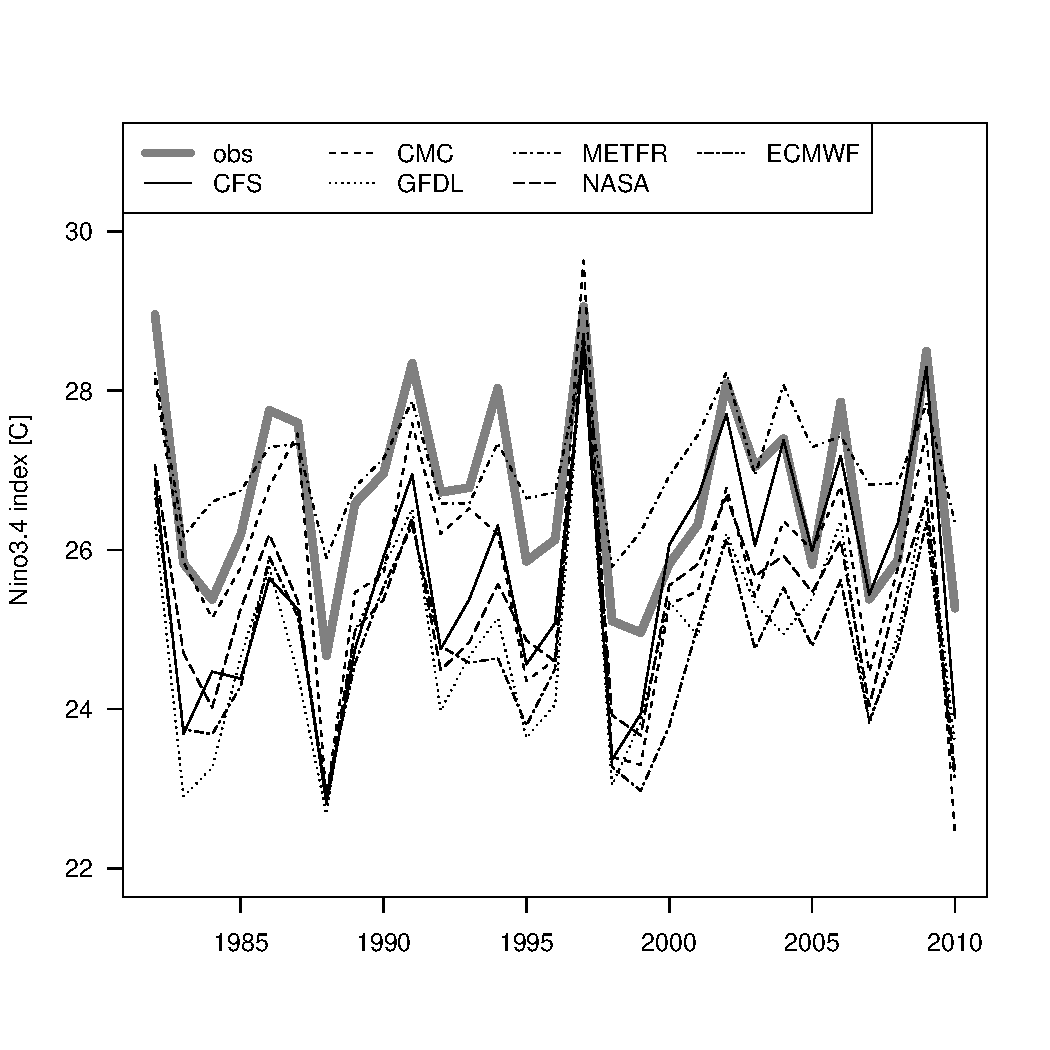
\includegraphics[width=.6\textwidth, page=1]{../R/enso_nao.pdf}\\
\includegraphics[width=.6\textwidth, page=2]{../R/enso_nao.pdf}
\end{center}
\caption{ENSO and NAO multi-model forecasts and observations.}
\label{fig:enso-nao}
\end{figure}


Below we summarise means, variances (using $1/n$ instead of $1/(n-1)$), and correlations of ENSO and NAO data:
\begin{center}
\begin{tabular}{c|ccccccc}
\textbf{ENSO statistics} &  obs  & cfs   &cmc  &gfdl    &mf  &nasa    &ec \\
\hline
mean &26.70 &25.64 &25.77 &24.89 &27.05 &25.29 &24.82 \\
stdev & 1.21 &1.41 &1.54 &1.30 &0.67 &1.19 &1.24\\
\end{tabular}

\begin{tabular}{c|ccccccc}
\textbf{ENSO correlations}      &obs  &cfs  &cmc &gfdl   &mf &nasa   &ec\\
\hline
obs  &1.00 &0.81 &0.89 &0.85 &0.87 &0.88 &0.91\\
cfs  & &1.00 &0.78 &0.89 &0.93 &0.89 &0.86\\
cmc  & & &1.00 &0.82 &0.83 &0.90 &0.91\\
gfdl & & & &1.00 &0.87 &0.93 &0.92\\
mf   & & & & &1.00 &0.90 &0.90\\
nasa & & & & & &1.00 &0.94\\
ec   & & & & & & &1.00
\end{tabular}
\end{center}



\begin{center}
\begin{tabular}{c|cccccc}
\textbf{NAO statistics} & obs  &ecmwf  &lodyn  &metfr    &mpi   &ukmo \\
\hline
mean &   0.6  &0.75  &0.70 &1.03  &0.74  &0.60 \\
stdev &  1.4 &0.14 &0.12 &0.16 &0.10 &0.14 \\
\end{tabular}

\begin{tabular}{c|cccccc}
\textbf{NAO correlations} &obs  &ecmwf &lodyn &metfr    &mpi  &ukmo\\
\hline
obs    &1.00 &-0.070  &0.03  &0.18  &0.019 &-0.14\\
ecmwf &  &1.000  &0.47  &0.23 &-0.006  &0.14\\
lodyn  &  &  &1.00  &0.16  &0.051  &0.06\\
metfr  &  &  &  &1.00 &-0.130  &0.09\\
mpi    & &  & &  &1.000 &-0.10\\
ukmo  &  &  &  & &  &1.00
\end{tabular}
\end{center}


\section{Optimal combination by multivariate analysis}

For statistical post-processing, it is necessary to make distributional assumptions about the joint behavior of forecasts and observations.
We will work under the assumption that forecasts and observations are jointly Normally distributed.
In particular, we assume that the observation $y_t$ and the vector of forecasts $\vec{x}_t = (x^{(1)}_t, \dots, x^{(M)}_t)'$ at time $t$ are jointly drawn from a multivariate Normal distribution with fixed parameters:
%
\begin{equation}
\left[\begin{matrix}y_t\\ \vec{x}_t\end{matrix} \right] \sim \mathcal{N}\left( \left[\begin{matrix}\mu_y \\ \vec{\mu}_x \end{matrix}\right], \left[ \begin{matrix}\Sigma_{yy} & \mat{\Sigma}_{yx} \\ \mat{\Sigma}_{xy} & \mat{\Sigma}_{xx} \end{matrix} \right]  \right).
\label{eq:jointdist}
\end{equation}
%
Draws at different times are assumed to be independent.
Any biases in mean and scale, and varying levels of correlation between forecasts and observations are encoded in the paramters $\mu$ and $\Sigma$ of the joint Normal distribution.
These parametric assumptions allow us to derive the optimal post-processing of ensemble means into a prediction for the observation.


Under the assumption of joint Normality, the conditional distribution of the observation, given specific values of the forecasts $\vec{x} = \vec{m}_t = (m_t^{(1)}, \dots, m_t^{(M)})'$, is a Normal distribution
%
\begin{equation}
p(y_t | \vec{x}_t = \vec{m}_t) = \mathcal{N}(\mu_{y|x}(\vec{m}_t), \Sigma_{y|x})
\label{eq:regrlemma}
\end{equation}
%
with conditional mean $\mu_{y|x}$ and conditional variance $\Sigma_{y|x}$ given by
%
\begin{align}
\mu_{y|x}(\vec{m}_t) & = \mu_{y} + \mat{\Sigma}_{yx} \mat{\Sigma}_{xx}^{-1} (\vec{m}_t - \vec{\vec{\mu}}_x)\label{eq:cond_mean}\\
\Sigma_{y|x} & = \Sigma_{yy} - \mat{\Sigma}_{yx} \mat{\Sigma}_{xx}^{-1} \mat{\Sigma}_{xy}
\end{align}
%
(c.f. Mardia et al 1995 ch 3). 
From eq. \ref{eq:cond_mean} it follows that the optimal combination of the $M$ forecasts $(m_t^{(1)},\dots,m_t^{(M)})$ into a single prediction $\hat{y}_t$ for the observation, is given by the linear function
\begin{equation}
\hat{y}_t = a + \sum_{m=1}^M w_m x^{(m)}_t
\label{eq:y_hat}
\end{equation}
%
where
%
\begin{align}
a & = \mu_y - \mat{\Sigma}_{yx} \mat{\Sigma}_{xx}^{-1} \vec{\mu}_x\label{eq:a}\\
w_m & = \mat{\Sigma}_{yx}(\mat{\Sigma}_{xx}^{-1})_{m}\label{eq:wm}.
\end{align}
%
Here $(\mat{\Sigma}_{xx}^{-1})_m$ denotes the $m$th column of the inverse of $\mat{\Sigma}_{xx}$.
Eq. \ref{eq:wm} shows that the weight of forecast $m$ in the combined prediction depends on the covariances of all forecasts with the observations, as well as the covariances of forecast $m$ with all the other forecasts.



In general the parameters of the Normal distribution are unknown, and have to be estimated from available tuples of past forecasts and observations.
We will look into the problem of parameter estimation later.
For the moment, we assume that the parameters $\vec{\mu}$ and $\mat{\Sigma}$ are known exactly.
Plugging in these values into equations \ref{eq:a} and \ref{eq:wm} then yields the overall mean $a$, the post-processing weights $w_m$, and the residual variance $\Sigma_{y|x}$. 
If we assume that the mean and covariance of the joint distribution of forecasts and observations are equal to the sample means and covariances of the ENSO data, we get

\begin{center}
\begin{tabular}{c|cccccc|c}
     $a$  &$w_{\mathrm{cfs}}$  &$w_{\mathrm{cmc}}$ &$w_{\mathrm{gfdl}}$   &$w_{\mathrm{mf}}$ &$w_{\mathrm{nasa}}$   &$w_{\mathrm{ec}}$      &$\Sigma_{y|x}$ \\
 -4.07  &-0.10   &0.33   &0.17   &0.66  &-0.16   &0.28   &0.19 
\end{tabular}
\end{center}

and if we plugin the sample means and covariances of the NAO data, we get

\begin{center}
\begin{tabular}{c|ccccc|c}
       $a$  &$w_{\mathrm{ecmwf}}$  &w$_{\mathrm{lodyn}}$  &w$_{\mathrm{metfr}}$    &w$_{\mathrm{mpi}}$   &w$_{\mathrm{ukmo}}$        &$\Sigma_{y|x}$ \\
-0.37 & -1.27  & 0.74  & 1.90  & 0.38 & -1.41  & 1.58
\end{tabular}
\end{center}


For simplicity, it is often preferred to combine models from different forecast centres by a democratic vote, where each model gets the same weight in the combination.
Such an equal-weights post-processingn scheme is equivalent to post-processing the multi-model mean (MMM); we combining all forecasts into the MMM first, and then fit the observation to the MMM by linear regression.


Given the multivariate Normal distribution of forecasts and observations (eq. \ref{eq:jointdist}), what is the optimal post-processing scheme for the multi-model mean (MMM), i.e., for equal-weights post-processing?
We use the following well-known result from Normal theory: If the vector $\vec{x}$ is a random variable $\vec{x}\sim \mathcal{N}(\vec{\mu}, \mat{\Sigma})$ then the linear form $\mat{A}\vec{x} \sim \mathcal{N}(\mat{A}\vec{\mu}, \mat{A}\mat{\Sigma}\mat{A}')$.
To combine the individual forecasts into the MMM, we set
%
\begin{equation}
\mat{A} = \left(\begin{matrix} 1 & 0 & \dots & 0 \\ 0 & \frac1M & \dots & \frac1M\end{matrix}\right),
\end{equation}
%
which transforms the vector of observations and forecasts into the 2-vector of observation and MMM.
We can then calculate the joint distribution of the observation and the MMM. 
From this joint distribution, we obtain the forecast distribution for the observation given the MMM, i.e., $p(y_t | \bar{x}_t = m_t)$, using eq.~\ref{eq:regrlemma}:
%
\begin{equation}
p(y_t|\bar{x}_t = \bar{m}_t) = \mathcal{N}\left(\mu_y + \frac{\Sigma_{y\bar{x}}}{\Sigma_{\bar{x}\bar{x}}} (\bar{m}_t - \mu_{\bar{x}}), \Sigma_{yy} - \frac{\Sigma_{\bar{x}y}^2}{\Sigma_{\bar{x}\bar{x}}}\right)
\end{equation}
%
where $\Sigma_{y\bar{x}}$, $\Sigma_{\bar{x}\bar{x}}$ and $\mu_{\bar{x}}$ are given by 
%
\begin{align}
\mu_{\bar{x}} & = \frac1M \sum_{m=1}^M \vec{\mu}_x^{(m)}\\
\Sigma_{\bar{x}\bar{x}} & = \frac{1}{M^2}\sum_{m=1}^M\sum_{m'=1}^M \mat{\Sigma}_{xx}^{(m,m')} \\
\Sigma_{y\bar{x}} & = \frac1M \sum_{m=1}^M \mat{\Sigma}_{yx}^{(m)}
\end{align}
%
Post-processing with equal weights is a simple linear regression with parameters $a$, $w_{MMM}$ and $\Sigma_{y|x}$ as in eq. \ref{eq:y_hat}.
Assuming the ENSO and NAO correlation structures, we get the following equal-weighting post-processing parameters 
%
\begin{center}
\begin{tabular}{c|ccc}
& $a$ & $w_{\mathrm{MMM}}$ & $\Sigma_{y|x}$ \\
\hline
\textbf{ENSO} & $2.32$ & $0.95$ & $0.24$ \\
\textbf{NAO} & $0.34$ & $0.34$ & $1.70$ 
\end{tabular}
\end{center}

For reference, we also consider the trivial post-processing scheme where the forecasts are ignored, and a climatological forecast is made for the observation.
The climatological forecast is equivalent to a post-processing with zero weights, i.e.
%
\begin{align}
\mu_{y|x} & = \mu_y\\
\Sigma_{y|x} & = \Sigma_{yy}
\end{align}



We consider the questions what is the potential benefit of using unequal weighting vs equal weighting for MMEs with a known correlation structure.
To address this, we calculate expected verification scores, in particular the expected squared error of the forecast mean (SQERR), the continuous ranked probability score (CRPS) and the logarithmic score (LOGS).
The corresponding equations for Normal forecast distributions are
%
\begin{align}
SQERR(\mathcal{N}(\mu_{y|x},\Sigma_{y|x}),y) & = (\mu_{y|x} - y)^2\label{eq:normal_sqerr}\\
CRPS(\mathcal{N}(\mu_{y|x},\Sigma_{y|x}),y) & = \sigma_{y|x}(2\varphi(z)+z(2\Phi(z)-1)-\pi^{-\frac12})\label{eq:normal_crps}\\
LOGS(\mathcal{N}(\mu_{y|x},\Sigma_{y|x}),y) & = \frac12(\log2\pi + \log\Sigma_{y|x} + z^2)\label{eq:normal_logs}
\end{align}
%
where $\sigma_{y|x} = \sqrt{\Sigma_{y|x}}$, $z=(y - \mu_{y|x})/\sigma_{y|x}$, and $\varphi$ and $\Phi$ are the pdf and cdf of the standard Normal distribution.
Eq. \ref{eq:normal_sqerr} is trivial, eq. \ref{eq:normal_crps} was given in \cite{gneiting2007} and eq. \ref{eq:normal_logs} follows from the distribution law of the Normal distribution.
The expectations of the above scores can be calculated analytically under the joint Normal assumption.


In all three post-processing scenarios (climatology, equal weights, unequal weights), the observation $y_t$ is assumed to have a Normal distribution $\mathcal{N}(\mu, \sigma^2)$, with constant forecast variance $\Sigma_{y|x}$, and a forecast mean $\mu_{y|x}$ that is either constant (climatological forecast) or depends on the values of the model forecasts (equal and unequal weighting).
To calculate the expected value of the score $S(\mathcal{N}(\mu,\sigma^2),y)$, we use conditional expectations:
%
\begin{equation}
E_{x,y}S\left[\mathcal{N}(\mu_{y|x},\Sigma_{y|x}),y\right] = E_x\left[ E_{y|x} S\left[\mathcal{N}(\mu_{y|x},\Sigma_{y|x}), y\right]\right]
\end{equation}
%
The inner expectation, taken over all possible values of the observation $y$ for a given value of the forecast $x$, is given by
%
\begin{align}
E_{y|x} \mathrm{SQERR} & = \Sigma_{y|x}\label{eq:esqerr}\\
E_{y|x} \mathrm{CRPS} & = \sqrt{\frac{\Sigma_{y|x}}{\pi}}\label{eq:ecrps}\\
E_{y|x} \mathrm{LOGS} & = \frac12\left( \log2\pi + \log\Sigma_{y|x} +1\right)\label{eq:elogs}
\end{align}
%
None of these expected scores depend on the particular value of $x$, because the forecast variance is constant in all three forecasting schemes.
Taking the expectation $E_x$ therefore leaves the expressions in eq. \ref{eq:esqerr}-\ref{eq:elogs} unchanged.


The expected score values assuming the ENSO and NAO correlation structures are:
%
\begin{center}
\begin{tabular}{cccc}
\textbf{ENSO} & SQERR & CRPS  & LOGS\\
clim    & 1.51 & 0.69 & 1.63\\
equal   & 0.24 & 0.28 & 0.71\\
unequal & 0.19 & 0.25 & 0.59\\
\hline
\textbf{NAO} & SQERR    & CRPS    & LOGS\\
clim    & 1.9636 & 0.79058 & 1.7563\\
equal   & 1.9630 & 0.79046 & 1.7562\\
unequal & 1.8244 & 0.76205 & 1.7196
\end{tabular}
\end{center}

For both settings, the unequal weighting performs better than equal weighting on average.
This result is expected because the correlations of the different models with the observation are different, and so the weights assigned to different forecasts should be different.
Since we are working under the assumption that all distributional parameters are known exactly, equal weighting leads to a worse forecast than unequal weighting.


The analysis illustrates the magnitudes of the potential improvement that we might get from using the optimal weighting with unequal weights as opposed to using the (sub-optimal) weighting with equal weights. 
For ENSO, the improvement of equal weighting over the climatology is very large for all scores, compared to the improvement of unequal weighting over equal weighting.
For NAO, all score improvements are tiny; but the improvement of unequal weighting over equal weighting is much larger than the improvement of equal weighting over the climatological forecast.

The improvements can be quantified by relative scores (skill scores) which we define here as the score differences between equal and unequal weighting, normalised by the score difference between climatological and unequal weighting:
%
\begin{equation}
S_{rel} = \frac{S_{equal} - S_{unequal}}{S_{clim} - S_{unequal}}
\end{equation}
%
The relative scores are given by
%
\begin{center}
\begin{tabular}{c|ccc}
& SQERR & CRPS &  LOGS \\
\hline
\textbf{ENSO} & 0.038 & 0.069 & 0.113 \\
\textbf{NAO} & 0.9957 & 0.9958 & 0.9959 
\end{tabular}
\end{center}

The relative improvements are vastly different between ENSO and NAO.
For ENSO, the scores achieved by equal weighting is relatively close the scores achieved by unequal weighting, but for NAO the equal weighting scores are (relatively) rarely better than the climatological scores.
The behavior of the different scores is similar for ENSO and NAO: The log score indicates the biggest relative improvement of unequal weighting over equal weighting, and the squared error the smallest.


The above analysis was based on highly idealised assumptions.
In general we do not know the parameters of the joint distribution of forecasts and observations exactly.
In general all we have is a finite sample of forecasts and observations.
We can make an assumption of joint Normality and independence and estimate the parameters.
In this case, the quality of our post-processed forecasts will also be affected by random errors due to the finiteness of the data set that is used for estimating the parameters.

\section{Equal vs unequal weighting based on finite training data}


\begin{figure}
\centering
\includegraphics[width=.7\textwidth, page=15]{../R/n-dependence.pdf}
\caption{Illustration of the random number experiment. The black and gray solid lines to the left of the dashed lines are ensemble means and observations in the training data set. These data are used to estimate the post-processing weights. A single set of forecasts is produced out of sample (open circles to the right of the dashed line), and post-processed into a predictive distribution function, using the parameters estimated from the training data set. This forecast distribution is compared with the out-of-sample verifying observation (gray square) using the squared error, the CRPS, and the Log score.}
\label{fig:illu}
\end{figure}


In this section, we perform random number experiments to study the effect of the finite hindcast size $n$ on how well the post-processing weights can be estimated, and how well the post-processed forecasts perform at predicting future observations.
We fix parameters $\vec{\mu}$ and $\mat{\Sigma}$ of a multivariate Normal distribution as in eq. \ref{eq:jointdist}, from which we draw $n$ independent samples of forecasts and observations.
These $n$ samples represent training data from which we wish to estimate post-processing weights.
We estimate the mean vector $\hat{\vec{\mu}}$ and the covariance matrix $\hat{\mat{\Sigma}}$ which we use to calculate the weights to post-process future forecasts.
Then we draw one more sample from the same multivariate distribution, which we use as a test case. 
That is, we get one additional set of forecasts $\vec{x}_{n+1}$ and a single verifying observation $y_{n+1}$.
We use the post-processing parameters $\hat{\vec{\mu}}$ and $\hat{\mat{\Sigma}}$ to transform the forecasts $\vec{x}_{n+1}$ into a predictive distribution for the observation $y_{n+1}$, using unequal weighting and equal weighting.
The forecasts are evaluated by the average SQERR, CRPS, and LOGS.
The random number experiment is illustrated in Fig. \ref{fig:illu}.
For every setting of $\vec{\mu}$, $\mat{\Sigma}$, and $n$, we repeat the random number experiment $10^6$ times, resulting in a collection of $10^6$ values of verification scores. 
The average scores are used to evaluate the of out-of-sample predictions of post-processing with equal and unequal weighting.


\begin{figure}
\begin{center}
\includegraphics[width=.6\textwidth, page=7]{../R/n-dependence.pdf}\\
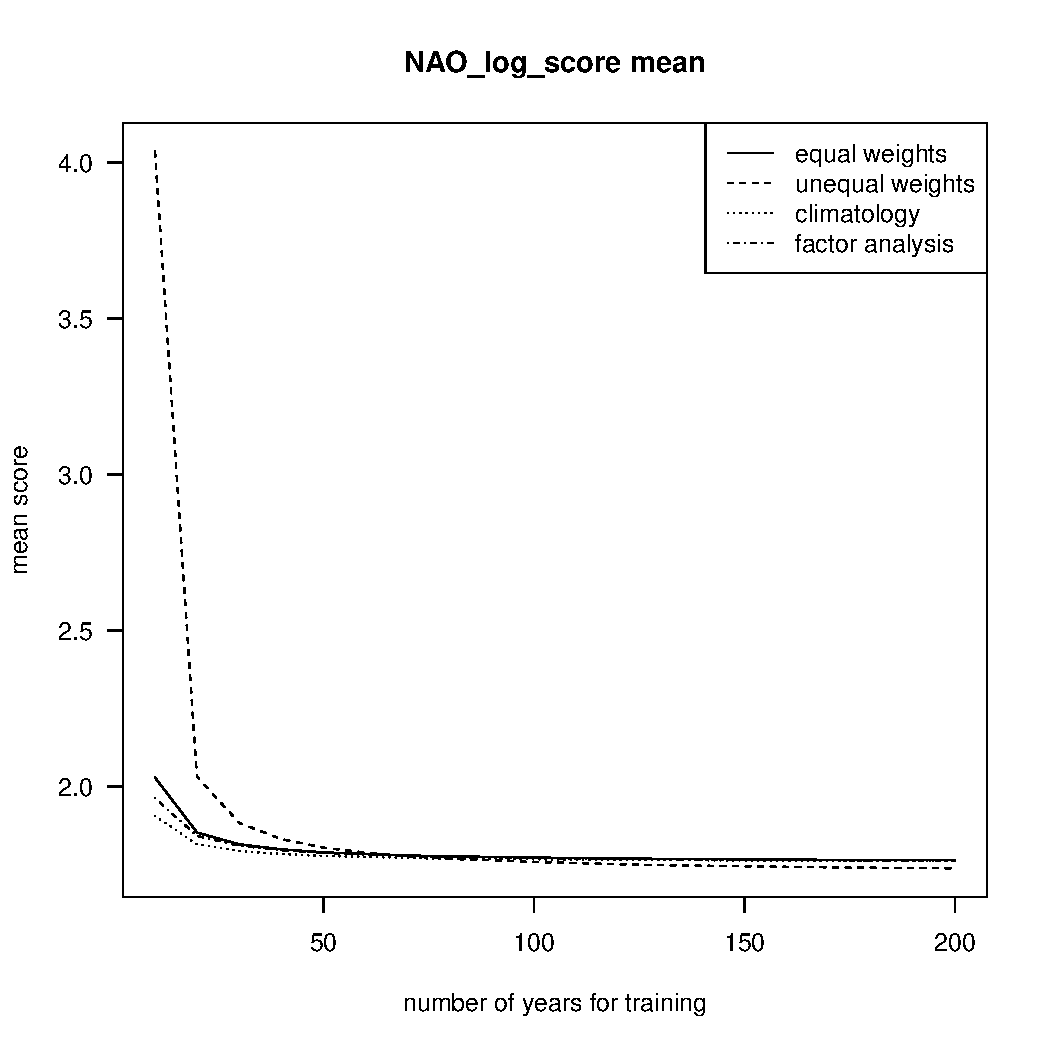
\includegraphics[width=.6\textwidth, page=1]{../R/n-dependence.pdf}
\end{center}
\caption{Out-of-sample mean log-scores achieved by post-processing with equal weights, unequal weights, and climatology as a function of the training sample size $n$. The upper panel is for simulated data using the mean and covariance matrix of the ENSO data, and the lower panel is for NAO. The equivalent plots for mean squared error and mean CRPS look similar.}
\label{fig:se_vs_n}
\end{figure}

Figure \ref{fig:se_vs_n} shows how the out-of-sample mean log-score behaves as a function of the training sample size $n$.
To simulate the MME forecast and observation data, we used the parameters $\vec{\mu}$ and $\mat{\Sigma}$ calculated for the NAO and ENSO seasonal prediction data sets.
We note the following:
%
\begin{enumerate}
\item For large sample sizes, unequal weighting outperforms climatology and equal weighting on average, as expected.
\item For small sample sizes, however, the expected score is smaller for post-processing with equal weights than with unequal weights.
For the ENSO parameters, equal weighting is better if the training sample size $n\le30$, and for the NAO setting, equal weighting is better on average if $n\le 60$.
\item For the NAO parameters and sample sizes $n \le 20$, unequal weighting is even outperformed by the climatological forecast  
\item The scores converge to a stable mean value at different rates: Climatology converges fastest, then equal weighting, then unequal weighting.
\item At large $n$, the magnitude of the improvement of unequal weighting over equal weighting is small compared to the improvement of equal weighting over climatology.
\item All the above conclusions hold for CRPS and SQERR as well (not shown). 
\end{enumerate}


These observations raise a number of questions about how seasonal MME's should be post-processed:
\begin{enumerate}
\item Given the small number of hindcast samples $n$ that we normally have for seasonal predictions, should we always prefer equal weighting over unequal weighting, even if we think that the different models are of different quality?
\item Given the small effect that we can expect from unequal weighting, is it worthwhile to pursue unequal weighting at all?
\item Given the large variability of values of the verification score, how likely are we to see an improvement from unequal weighting for a given forecast?
\end{enumerate}


The first two questions are subjective and have to judged on a case by case basis, perhaps using simulation studies as we did above.
The third question can be answered for our simulation study.
For each foreacst instance, we get two post-processed forecasts for the same observation, one based on equal weighting and one based on unequal weighting.
Each forecast obtains a certain value of the verification score.
On any particular forecast instance, equal weighting is either better or worse than unequal weighting.
We can now ask the questions ``How often does unequal weighting produce a better forecast than equal weighting''?


\begin{figure}
\begin{center}
\includegraphics[width=.6\textwidth, page=14]{../R/n-dependence.pdf}\\
\includegraphics[width=.6\textwidth, page=13]{../R/n-dependence.pdf}\\
\end{center}
\caption{Fraction of cases where the forecast produced with unequal weighting outperforms the forecast produced with equal weighting as a function of the training sample size $n$. Upper panel is for data with ENSO correlation structure, lower panel is for NAO.}
\label{fig:prob_impr}
\end{figure}

In Figure \ref{fig:prob_impr}, the fraction of cases where unequal weighting improves upon equal weighting is shown as a function of the training sample size $n$.
We find that for small sample sizes, equal weighting is more likely than not to produce a better forecast than unequal weighting.
For larger sample sizes, unequal weighting is more likely to produce a better forecast than equal weighting.
But even for large training sample sizes, there is still a considerable fraction of cases, where equal weighting outperforms unequal weighting.
Furthermore, the 3 scoring rules SQERR, CRPS, and LOGS behave markedly differently.
The logarithmic score is much more likely to show an improved forecast due to unequal weightingthan the other two scores.
The mean squared error is least likely to indicate an improvement of unequal over equal weighting.

\section{Conclusions}

We have presented analytical results and a simulation exercise to study the expected improvement of unequal weighting over equal weighting for post-processing seasonal forecasts.
We found that unequal weighting is asymptotically superior to equal weighting, in a sense that expected verification scores obtained by unequal weighting are always better than for equal weighting, given that the parameters of the joint distribution of forecasts and observations are known.

However, for the examples considered the potential improvement in scores is rather small.
Furthermore, the improvement depends on the availability of a sufficiently large record of past forecasts and observations from which the post-processing weights can be estimated. 
If the number of training samples is too small, the simpler post-processing strategy with equal weights outperforms post-processing with unequal weights.
Lastly, the internal variability of the forecast and observation data does not guarantee that the optimal post-processing method with outperforms a sub-optimal method on any given forecast instance.

These results can be used to guide the operational decision as to whether a democratic vote (equal weighting) should be used to combine several model forecasts into a single forecast, or whether more complicated combination schemes based on unequal weighting should be pursued.

\end{document}

